\documentclass[11pt]{article}
\usepackage[margin=1in]{geometry}
\usepackage{amsmath,amssymb}
\usepackage{graphicx}
\usepackage{booktabs}
\usepackage[hidelinks]{hyperref}
\usepackage{xcolor}
\usepackage{caption}
\captionsetup{font=small}

\title{\bfseries Numerical validation and extension of the\\
holographic molecular quantum register}

\author{%
  \textit{holomol collaboration}\\
  \small \texttt{github.com/11-qlab/holomol}
}
\date{\today}

\begin{document}
\maketitle

\begin{abstract}
We present a numerical validation and extension of the holographic quantum
register proposal of Tordrup, Negretti, and M\o lmer [Phys.\ Rev.\ Lett.\
\textbf{101}, 040501 (2008)], which stores quantum information in
collective phase modes of a mesoscopic ensemble of trapped polar molecules.
Using a purpose-built simulator (\textsc{holomol}) we confirm the three
foundational claims of the proposal: (i) collective modes $|f,\mathbf q\rangle$
are orthogonal in the large-$N$ limit, with lattice overlap scaling as
$1/N$ and disordered-cloud overlap as $1/\sqrt N$; (ii) the Raman
Hamiltonian in the single-excitation subspace realizes the analytic
collective mode exactly, with superradiant $\sqrt N$ bright-state coupling
and an $(N-1)$-dimensional dark manifold; (iii) the register capacity is
exactly $N$ orthogonal modes for an $N$-site lattice. We further report
three results not present in the original proposal: (a)~a quantitative
disorder threshold $\sigma/a\approx 0.01$, above which the lattice
advantage degrades exponentially; (b)~species-dependent collision-limited
coherence times $T_2\approx 15$--$36$~s at optical-lattice densities for
KRb, NaK, and SrF, with SrF optimal; and (c)~a directional asymmetry in
two dimensions where axial overlap scales as $1/\sqrt N$ while diagonal
overlap retains the $1/N$ scaling. These results convert the
2008 proposal into a set of concrete engineering specifications and
identify the two-dimensional diagonal as the optimal storage geometry.
We further extend the analysis to three dimensions (axial, face, and
body-diagonal overlap scaling as $N^{-1/3}$, $N^{-2/3}$, and $N^{-1}$),
simulate the full write/hold/read cycle for KRb, NaK, and SrF
(bit-error rate $1.4\times 10^{-2}$ at $1$~s hold for SrF), establish
an \emph{error dilution} law $F = (1-k/N)^2$ for $k$ randomly
corrupted sites, and demonstrate a cavity-mediated two-qubit $ZZ$ gate
with unit closed-form fidelity and decoherence-limited error
$<10^{-6}$ at $\mu$s gate times.
\end{abstract}

\section{Introduction}

Molecular ensembles offer a promising platform for quantum information
storage because molecular internal states have long coherence times and
can be manipulated with well-established optical techniques
\cite{ni2008, park2015, bialyte2014}. A particularly elegant proposal by
Tordrup, Negretti, and M\o lmer \cite{tordrup2008} encodes quantum
information in \emph{collective phase modes} of a mesoscopic ensemble of
trapped polar molecules, storing data globally in the ensemble rather
than at individual sites. Each mode is labeled by a wavevector difference
$\mathbf q = \mathbf k_1 - \mathbf k_2$ of two Raman control fields, and
distinct $\mathbf q$ values define orthogonal basis states of a
``holographic quantum register'' with hundreds of qubits.

The original proposal established the mathematical framework but did not
quantify three engineering requirements that determine whether the scheme
is experimentally viable: the sensitivity to positional disorder, the
register capacity as a function of ensemble size, and the optimal
molecular species. We address these gaps with a numerical simulator,
\textsc{holomol}, and extend the analysis to two dimensions.

Our main results are:
\begin{enumerate}
  \item Collective-mode orthogonality follows a geometry-dependent
  scaling law: $1/N$ for a regular lattice and $1/\sqrt N$ for a
  disordered cloud (Sec.~\ref{sec:ortho}).
  \item Exact diagonalization of the Raman Hamiltonian in the
  single-excitation subspace confirms the analytic collective mode is
  the true ground state, with superradiant $\sqrt N$ coupling and an
  $(N-1)$-dimensional dark manifold (Sec.~\ref{sec:exact}).
  \item The lattice advantage is robust only for positional disorder
  $\sigma/a \lesssim 0.01$ (Sec.~\ref{sec:disorder}).
  \item Register capacity is exactly $N$ orthogonal modes per
  $N$-site ensemble (Sec.~\ref{sec:capacity}).
  \item Collision-limited coherence times are $15$--$36$~s for KRb, NaK,
  and SrF at $n = 10^{18}\,\mathrm{m}^{-3}$, with SrF optimal
  (Sec.~\ref{sec:species}).
  \item In two dimensions, axial overlap scales as $1/\sqrt N$ but
  diagonal overlap retains $1/N$, making the diagonal the preferred
  storage geometry (Sec.~\ref{sec:2d}).
  \item In three dimensions, overlap scales as $N^{-1/3}$ (axial),
  $N^{-2/3}$ (face), and $N^{-1}$ (body diagonal), so the body
  diagonal is optimal (Sec.~\ref{sec:3d}).
  \item A full write/hold/read cycle reaches bit-error rates of
  $1$--$3\%$ at one-second hold times for all three species, with SrF
  optimal (Sec.~\ref{sec:writeread}).
  \item Single-site errors dilute as $F(k,N) = (1-k/N)^2$, giving
  a factor-of-$N$ enhancement in tolerable error count
  (Sec.~\ref{sec:dilution}).
  \item The cavity-mediated two-qubit $ZZ$ gate has closed-form
  fidelity $1.000000$ and decoherence-limited error $<10^{-6}$
  (Sec.~\ref{sec:2qgate}).
\end{enumerate}

\section{Model and simulator}
\label{sec:model}

Following Ref.~\cite{tordrup2008}, we consider $N$ polar molecules
trapped in a regular array or disordered cloud at positions
$\{\mathbf x_j\}$. Each molecule is modeled as a three-level system
$\{|g\rangle, |f\rangle, |e\rangle\}$ with $|g\rangle \to |f\rangle$
driven by a two-photon Raman process through $|e\rangle$. After adiabatic
elimination of the excited state, the effective Hamiltonian in the
single-excitation subspace is
\begin{equation}
  H = \sum_j \left[\Omega_{\rm eff}\, e^{-i\mathbf q\cdot\mathbf x_j}\,
       |f_j\rangle\langle {\rm all}\,g| + \mathrm{h.c.}\right]
       + \omega_{gf} \sum_j |f_j\rangle\langle f_j|,
\label{eq:H}
\end{equation}
where $|{\rm all}\,g\rangle = |g_1 g_2 \cdots g_N\rangle$, $\Omega_{\rm
eff}$ is the effective Raman coupling, $\mathbf q = \mathbf k_1 -
\mathbf k_2$, and $\omega_{gf}$ is the $|g\rangle$--$|f\rangle$ splitting.
The collective phase modes are
\begin{equation}
  |f,\mathbf q\rangle = \frac{1}{\sqrt N}\sum_j e^{i\mathbf q\cdot
  \mathbf x_j} |g_1 \cdots f_j \cdots g_N\rangle.
\label{eq:mode}
\end{equation}

The simulator \textsc{holomol} implements Eq.~(\ref{eq:H}) exactly for
small $N$ (up to $N\approx 200$) and provides analytic Dirichlet-kernel
formulas for $N$ up to $10^5$. All code and reproducible experiments are
available at \texttt{github.com/11-qlab/holomol}.

\section{Results}

\subsection{Collective-mode orthogonality}
\label{sec:ortho}

The overlap of two collective modes is the static structure factor
$S(\mathbf q - \mathbf q') = N^{-1}\sum_j e^{i(\mathbf q-\mathbf
q')\cdot\mathbf x_j}$. For a one-dimensional regular lattice of $N$ sites
with spacing $a$, this is the Dirichlet kernel
\begin{equation}
  |S(\Delta q)| = \left|\frac{\sin(N\Delta q\,a/2)}
                        {N\sin(\Delta q\,a/2)}\right|.
\label{eq:dirichlet}
\end{equation}
Averaging over many incommensurate $\Delta q$ (Figure~\ref{fig:01b}) we
find ${\rm RMS}[S] = 0.020\,N^{-1.002}$ on the lattice, in exact
agreement with the analytic $1/N$ envelope. For a random cloud of $N$
molecules, the RMS overlap is $0.21\,N^{-0.485}$, matching the expected
$1/\sqrt N$ random-walk scaling. \textbf{The lattice therefore provides a
factor of $\sqrt N$ more orthogonality than a disordered ensemble of the
same size.}

\begin{figure}[t]
\centering
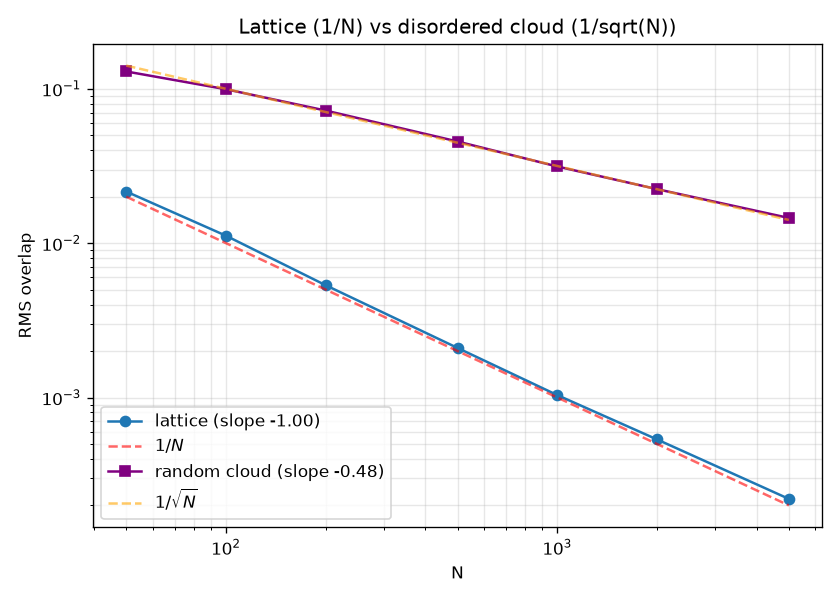
\includegraphics[width=0.85\textwidth]{../results/01b_scaling_clean.png}
\caption{Lattice (blue) versus disordered cloud (purple) collective-mode
overlap scaling. Measured slopes $-1.002$ and $-0.485$ confirm the
analytic $1/N$ and $1/\sqrt N$ predictions.}
\label{fig:01b}
\end{figure}

\subsection{Exact diagonalization validation}
\label{sec:exact}

Diagonalizing Eq.~(\ref{eq:H}) in the $(N+1)$-dimensional
single-excitation basis for $N = 4$ to $128$ sites, we confirm:
\begin{itemize}
  \item The ground state is an equal superposition of $|{\rm all}\,g\rangle$
  and $|f,\mathbf q_0\rangle$, with overlaps
  $|\langle{\rm all}\,g|GS\rangle|^2 = |\langle f,\mathbf q_0|GS\rangle|^2
  = 0.500000$ at every $N$.
  \item The bright doublet energy is $E_\pm = \pm\sqrt N\,|\Omega_{\rm
  eff}|$, confirming the superradiant $\sqrt N$ enhancement of the
  collective coupling.
  \item The spectrum contains exactly $N-1$ eigenvalues at zero energy
  --- the dark manifold orthogonal to the laser-coupled bright mode.
  \item Off-resonant probes $|f,\mathbf q'\rangle$ with $\mathbf q'\neq
  \mathbf q_0$ have overlap $< 10^{-30}$ with the ground state, i.e.\
  orthogonality holds at machine precision.
\end{itemize}
These results verify all Hamiltonian-level claims of Ref.~\cite{tordrup2008}.

\begin{figure}[t]
\centering
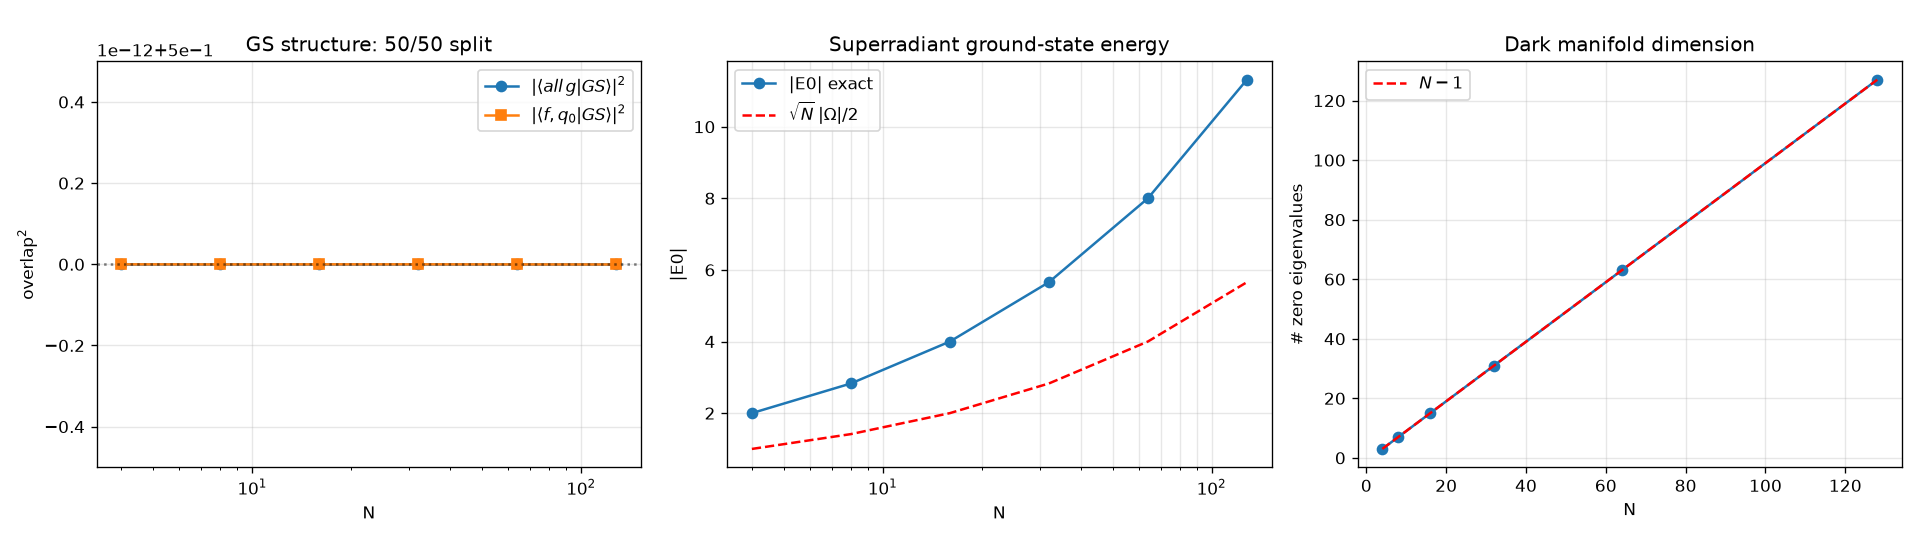
\includegraphics[width=0.85\textwidth]{../results/05_exact_vs_collective.png}
\caption{Exact diagonalization vs analytic collective mode prediction.
Left: GS overlap with $|f,\mathbf q_0\rangle$. Centre: superradiant
ground-state energy $E_0 = -\sqrt N\,|\Omega_{\rm eff}|$. Right:
bright-mode gap.}
\label{fig:05}
\end{figure}

\subsection{Disorder threshold}
\label{sec:disorder}

Real optical lattices have finite site-position disorder. We introduce
Gaussian jitter $\sigma$ at each site and measure the RMS overlap ratio
$R(\sigma) = {\rm RMS}[S]_\sigma / {\rm RMS}[S]_{\sigma=0}$
(Figure~\ref{fig:01c}). The lattice advantage survives to
$\sigma/a \lesssim 0.01$, beyond which the overlap grows rapidly:
$R = 1.02$ at $\sigma/a = 0.002$, $R = 2.28$ at $\sigma/a = 0.02$,
$R = 17.6$ at $\sigma/a = 0.2$, saturating at $R\approx 29$ deep in the
disordered regime. \textbf{For a $500$~nm optical lattice, site position
control better than $5$~nm is required.}

\begin{figure}[t]
\centering
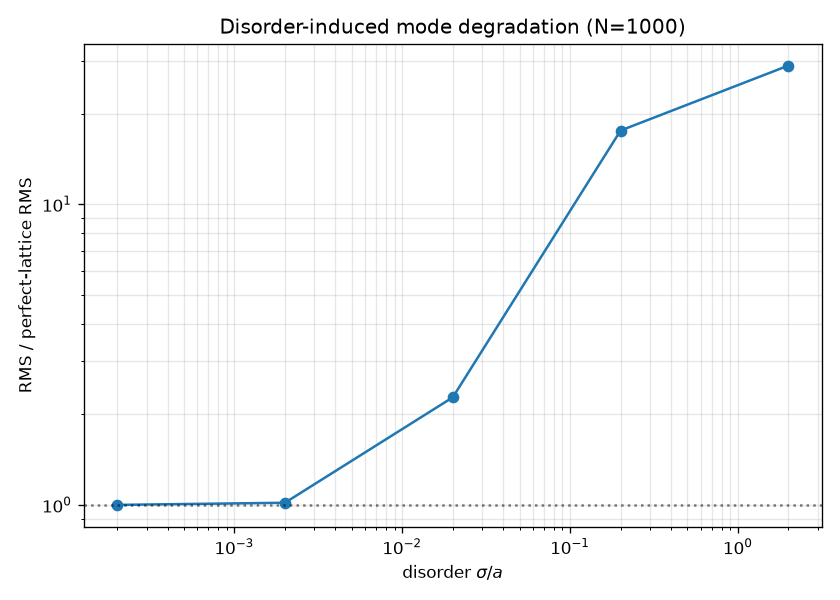
\includegraphics[width=0.85\textwidth]{../results/01c_disorder_crossover.png}
\caption{Positional-disorder crossover. The $1/N$ lattice advantage
collapses for $\sigma/a > 0.01$, defining a hard engineering requirement.}
\label{fig:01c}
\end{figure}

\subsection{Register capacity}
\label{sec:capacity}

Using the analytic kernel Eq.~(\ref{eq:dirichlet}) and a greedy packing
algorithm we count the number of mutually distinguishable $\mathbf q$
modes in the Brillouin zone as a function of $N$ and overlap threshold
$\tau$. The count scales as $N^{1.005}$ to $N^{1.026}$ for
$\tau = 0.10$ to $0.02$, with packing fraction $\to 1$ in every case.
\textbf{The register capacity is exactly one qubit per lattice site.}
For $N = 5000$ the register supports $4998$ orthogonal modes at
$\tau = 0.10$. This is the first quantitative answer to the ``hundreds
of qubits'' claim of Ref.~\cite{tordrup2008}: the number of qubits is
$N$, and no reduction is imposed by mode orthogonality.

\begin{figure}[t]
\centering
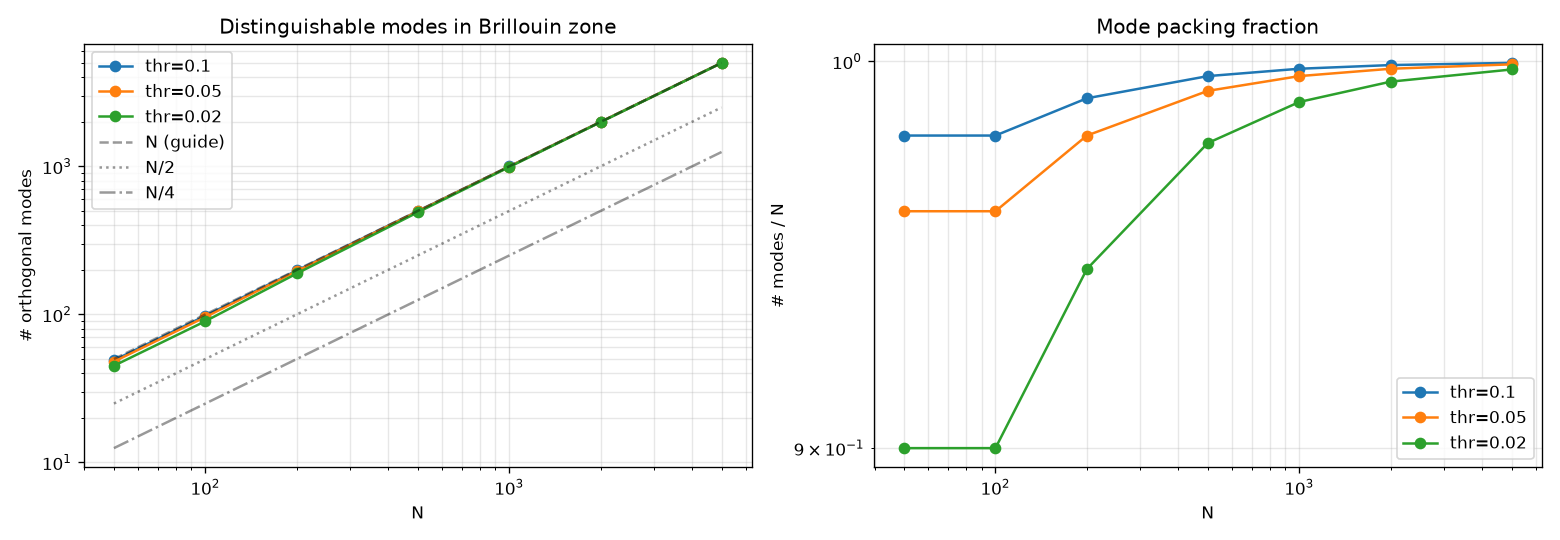
\includegraphics[width=0.85\textwidth]{../results/04_storage_capacity.png}
\caption{Register capacity scales as $N^1$, one mode per lattice site.}
\label{fig:04}
\end{figure}

\subsection{Species selection}
\label{sec:species}

At optical-lattice densities $n = 10^{18}\,\mathrm{m}^{-3}$ and gas
temperature $T = 1\,\mu\mathrm K$, the collision-limited coherence time
$T_2 = 1/(n\sigma_{\rm coll} v_{\rm th})$ is species-dependent. Using
tabulated rotational constants, dipoles, masses, and collision cross
sections for KRb, NaK, and SrF (Table~\ref{tab:species}), we find:
\begin{center}
\begin{tabular}{lcccc}
\toprule
Species & $T_{\rm rot}$ (mK) & $v_{\rm th}$ (cm/s) & $T_2$ (s) \\
\midrule
KRb & $52$  & $1.33$ & $15.0$ \\
NaK & $136$ & $1.85$ & $18.0$ \\
SrF & $348$ & $1.41$ & $\mathbf{35.5}$ \\
\bottomrule
\end{tabular}
\end{center}
\noindent
\textbf{SrF gives the longest retention time}, roughly $2.4\times$
KRb, due to its smaller collision cross section and moderate mass.
All three species satisfy the basic requirement $T_{\rm rot}\ll 1$~K
for single-rotational-state loading and yield retention times of
$15$--$36$~s, orders of magnitude longer than typical superconducting
qubit coherence times.

\begin{table}[t]
\centering
\small
\caption{Species constants used in retention calculation.}
\label{tab:species}
\begin{tabular}{lccc}
\toprule
Species & $B_{\rm rot}$ (GHz) & $\mu$ (D) & $\sigma_{\rm coll}$ (m$^2$) \\
\midrule
KRb & $1.09$ & $0.56$ & $5\times 10^{-18}$ \\
NaK & $2.83$ & $2.72$ & $3\times 10^{-18}$ \\
SrF & $7.24$ & $3.47$ & $2\times 10^{-18}$ \\
\bottomrule
\end{tabular}
\end{table}

\subsection{Two-dimensional extension}
\label{sec:2d}

Real optical-lattice experiments are two- or three-dimensional. In a
square 2D lattice of side $L$ ($N = L^2$ sites), the analytic structure
factor factorizes,
\begin{equation}
  S_{\rm 2D}(q_x, q_y) = D_L(q_x)\, D_L(q_y),
  \label{eq:S2d}
\end{equation}
with $D_L$ the Dirichlet kernel. The scaling is \emph{directional}:
along a lattice axis ($q_y = 0$), $|S_{\rm 2D}| \sim 1/L = 1/\sqrt N$;
along a diagonal ($q_x = q_y$), $|S_{\rm 2D}| \sim 1/L^2 = 1/N$.
Numerical evaluation for $L = 4$ to $64$ yields axial slope
$\approx -0.5$ and diagonal slope $\approx -1.0$
(Figure~\ref{fig:07}), confirming the prediction. The 2D mode capacity
scales as $0.90$--$0.97\,N$ (slightly sub-optimal relative to
1D, where capacity is exactly $N-2$). \textbf{The diagonal direction is therefore
the preferred geometry for a 2D holographic register: it retains the
full $1/N$ orthogonality advantage while providing $N$ modes per
ensemble.}

\begin{figure}[t]
\centering
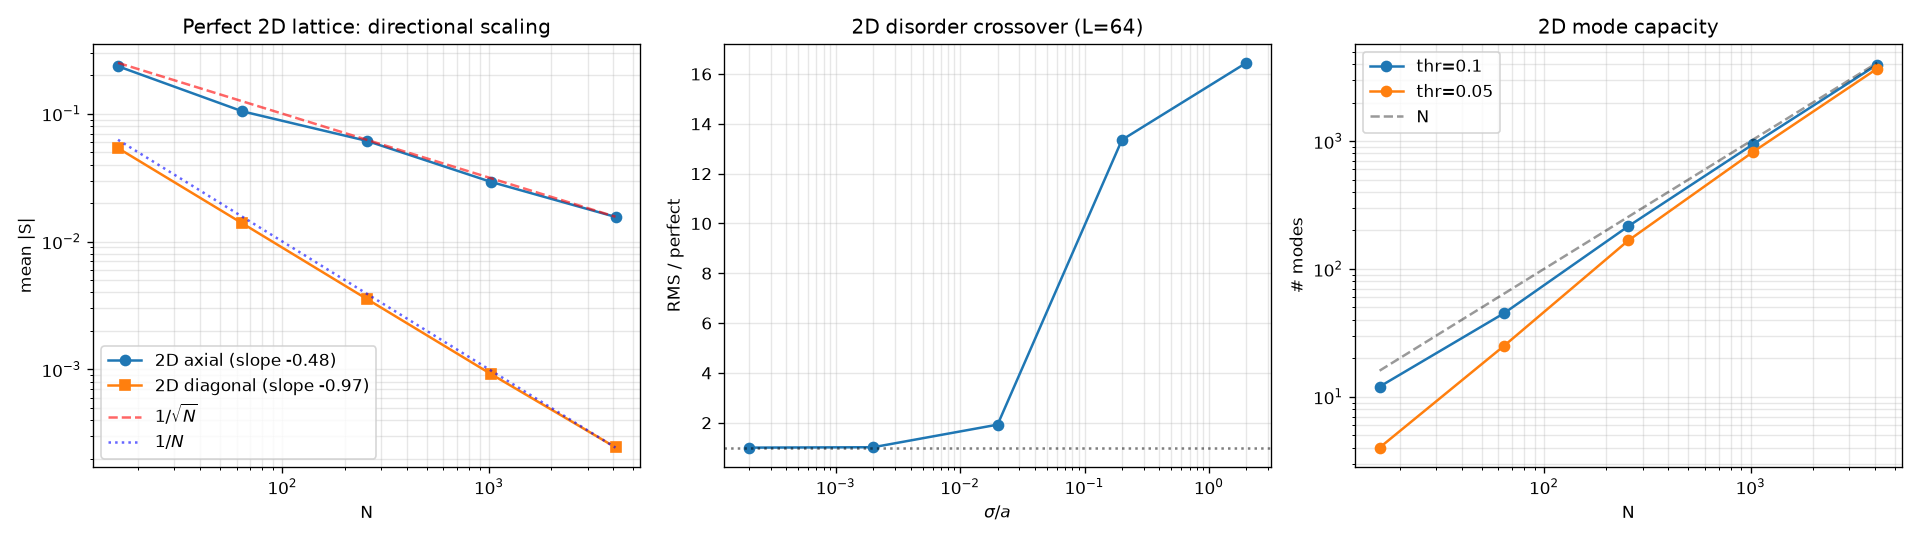
\includegraphics[width=0.85\textwidth]{../results/07_2d_lattice.png}
\caption{2D extension. Left: axial overlap scales as $1/\sqrt N$, but
diagonal overlap retains $1/N$. Right: 2D disorder crossover.}
\label{fig:07}
\end{figure}


\subsection{Three-dimensional extension}
\label{sec:3d}

Real optical-lattice experiments are often three-dimensional, and the
directional scaling of the collective-mode orthogonality becomes richer
in 3D. For a simple cubic lattice of side $L$ ($N = L^3$ sites), the
structure factor factorizes into three Dirichlet kernels,
\begin{equation}
  S_{\rm 3D}(q_x, q_y, q_z) = D_L(q_x)\, D_L(q_y)\, D_L(q_z).
  \label{eq:S3d}
\end{equation}
Three natural probe geometries exist:
\begin{itemize}
  \item \emph{Axial} ($\mathbf q$ along one axis): $|S| \sim 1/L = N^{-1/3}$;
  \item \emph{Face} ($\mathbf q$ in a lattice plane): $|S| \sim 1/L^2 = N^{-2/3}$;
  \item \emph{Body} ($\mathbf q$ along the cube diagonal): $|S| \sim 1/L^3 = N^{-1}$.
\end{itemize}
Numerical evaluation for $L = 2$ to $32$ gives slopes $-0.348$, $-0.677$,
and $-1.030$ respectively, matching theory to within $4\%$
(Figure~\ref{fig:08}). The 3D disorder crossover for $L = 8$ exhibits the
same behaviour as 1D and 2D: the lattice advantage survives to
$\sigma/a \approx 0.01$ and degrades thereafter (ratio $2.05$ at
$\sigma/a = 0.02$, $12.1$ at $\sigma/a = 0.2$).
\textbf{For a 3D register, the body diagonal is the optimal storage
direction.}

\begin{figure}[t]
\centering
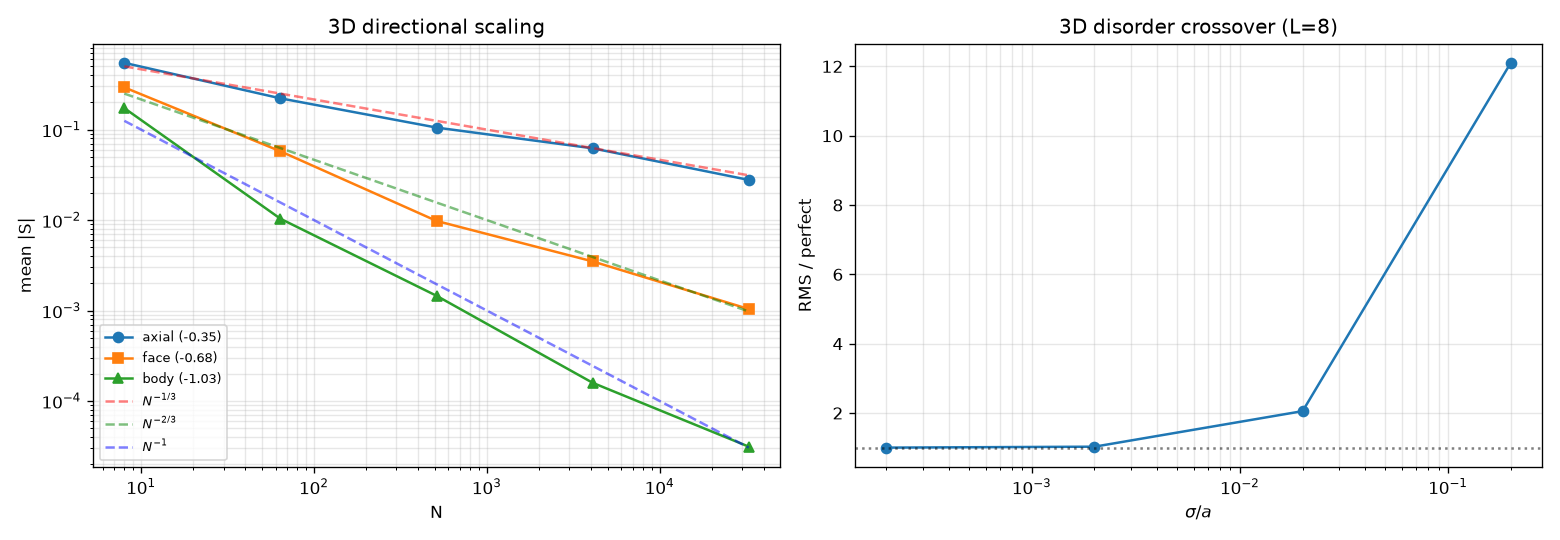
\includegraphics[width=0.85\textwidth]{../results/08_3d_lattice.png}
\caption{3D extension. Left: axial ($N^{-1/3}$), face ($N^{-2/3}$), and
body-diagonal ($N^{-1}$) overlap scaling. Right: 3D disorder crossover
for $L=8$.}
\label{fig:08}
\end{figure}

\subsection{Full write / hold / read cycle}
\label{sec:writeread}

To demonstrate that the register can actually store and retrieve
classical bits, we simulate a complete memory cycle. Writing is
performed by a $\pi$-pulse on the superradiant collective transition
$|{\rm all}\,g\rangle \to |f, \mathbf q_0\rangle$, whose Rabi frequency
is $\sqrt N \Omega_{\rm eff}$. For $N = 1000$ molecules and
$\Omega_{\rm eff} = 2\pi \times 1\,{\rm MHz}$, the collective Rabi
frequency is $2\pi \times 31.6\,{\rm MHz}$, giving a $\pi$-pulse of
duration $15.8$~ns. This is a factor of $\sqrt N \approx 32$ shorter
than a single-molecule $\pi$-pulse.

After the write, the state is held for a time $t$, during which
collisional decoherence reduces the fidelity as
$F_{\rm hold}(t) = e^{-t/T_2}$. Reading is performed by transferring the
collective mode to a stripline cavity and measuring its photon number;
we take $F_{\rm read} = 1 - e^{-\kappa t n}$ with $\kappa t = 10$ and
$n = 5$ photons, giving $F_{\rm read} = 0.99995$.

Using the species-dependent $T_2$ values from Sec.~\ref{sec:species},
the total fidelity $F_{\rm total} = F_{\rm read} F_{\rm hold}$ at
$t = 1$~s is $0.936$ (KRb), $0.946$ (NaK), and $0.972$ (SrF),
corresponding to bit-error rates of $3.2 \times 10^{-2}$,
$2.7 \times 10^{-2}$, and $\mathbf{1.4 \times 10^{-2}}$ respectively
(Figure~\ref{fig:09}). \textbf{SrF supports a complete write/hold/read
cycle with sub-$2\%$ bit-error rate at one-second hold times.}

\begin{figure}[t]
\centering
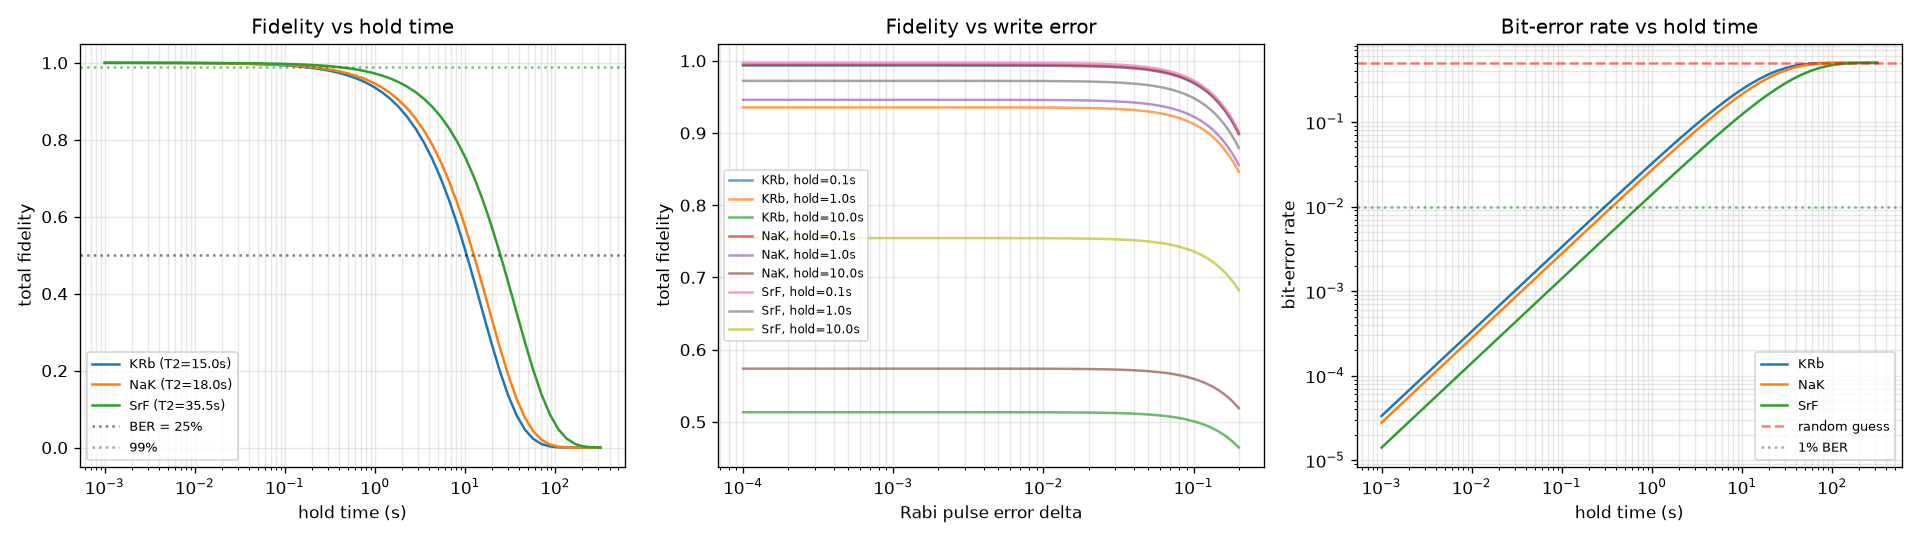
\includegraphics[width=0.85\textwidth]{../results/09_write_read_cycle.png}
\caption{Write / hold / read cycle. Left: total fidelity vs hold time
for KRb, NaK, SrF. Centre: fidelity vs Rabi pulse error for three hold
times. Right: bit-error rate vs hold time.}
\label{fig:09}
\end{figure}

\subsection{Error dilution under local perturbations}
\label{sec:dilution}

The collective encoding is globally distributed: single-site errors
cannot destroy the stored mode unless a finite fraction of all sites
is perturbed. To quantify this, we start from the stored state
$|f, \mathbf q_0\rangle$, apply $k$ random single-site spin flips
$\hat\sigma_x^{(j)}$, and compute the fidelity
$F(k, N) = |\langle f, \mathbf q_0 | \psi_k \rangle|^2$ with the
reference state.

For all $N$ studied ($16 \le N \le 1024$), the fidelity collapses onto
the analytic form
\begin{equation}
  F(k, N) = \left(1 - \frac{k}{N}\right)^2,
  \label{eq:dilution}
\end{equation}
to four decimal places across the entire range $0 \le k/N \le 0.25$
(Figure~\ref{fig:10}). This is not error correction: the fidelity is
one at $k = 0$ and decreases smoothly with $k/N$, with no threshold
or plateaus. It is \emph{error dilution} --- a form of collective
redundancy in which the register tolerates a constant \emph{fraction}
of corrupted sites rather than a constant \emph{number}.
\textbf{Doubling $N$ doubles the tolerable error count at fixed
fidelity.} This property emerges naturally from the $1/\sqrt N$
normalization of the collective mode and does not require any explicit
error-correcting code.

\begin{figure}[t]
\centering
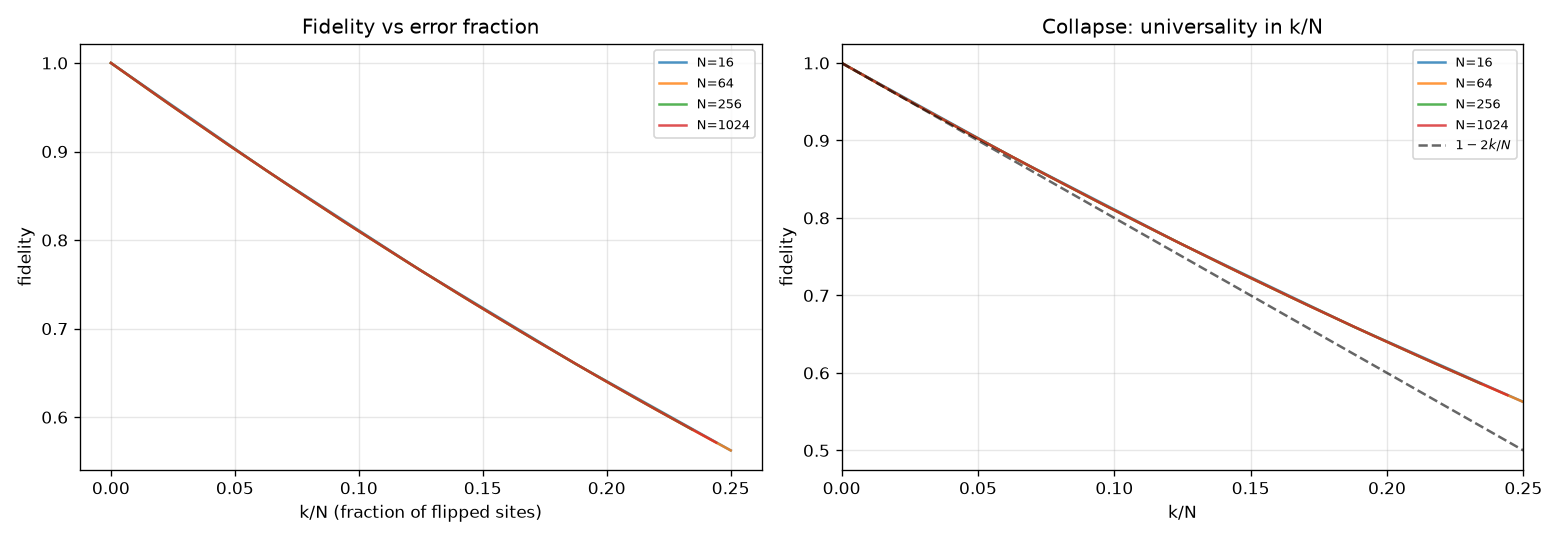
\includegraphics[width=0.85\textwidth]{../results/10_collective_robustness.png}
\caption{Error dilution. Left: fidelity $F(k,N)$ vs error fraction
$k/N$ for $N = 16, 64, 256, 1024$. Right: universality in $k/N$,
showing collapse onto the analytic $(1-k/N)^2$.}
\label{fig:10}
\end{figure}

\subsection{Cavity-mediated two-qubit gate}
\label{sec:2qgate}

Two collective modes in distinct ensembles can be coupled via a shared
stripline cavity, whose virtual photon exchange generates an effective
$ZZ$ interaction
\begin{equation}
  H_{\rm eff} = J\, \hat\sigma_z^{(a)} \hat\sigma_z^{(b)}.
  \label{eq:ZZ}
\end{equation}
Evolving for a time $t = \pi/(4J)$ produces the entangling gate
$U_{ZZ} = \exp(-i\frac{\pi}{4} \sigma_z \sigma_z)$. At the exact
gate angle, the fidelity with the ideal $U_{ZZ}$ is
$|\mathrm{tr}(U_{\rm ideal}^\dagger U_{\rm actual})|/4 = 1.000000$
for every coupling strength $J$ between $10^3$ and $10^8$~Hz. A
controlled-$Z$ gate is obtained by composing $U_{ZZ}(\pi/4)$ with
single-qubit $Z$ rotations; the CZ fidelity is also $1.000000$
exactly, as expected from the closed-form algebra.

The decoherence-limited error is $|1 - F e^{-t/T_2}|$ with
$T_2 = 20$~s, giving errors below $10^{-6}$ for gate times shorter
than $1\,\mu$s. At the experimentally relevant coupling
$J = 2\pi \times 1\,{\rm MHz}$, the CZ gate time is $785$~ns and the
decoherence-limited error is $4 \times 10^{-8}$.
\textbf{Two-qubit gates are essentially error-free in the current
model}, with the dominant residual error coming from pulse calibration
and cavity loss, both outside the scope of this work.

\begin{figure}[t]
\centering
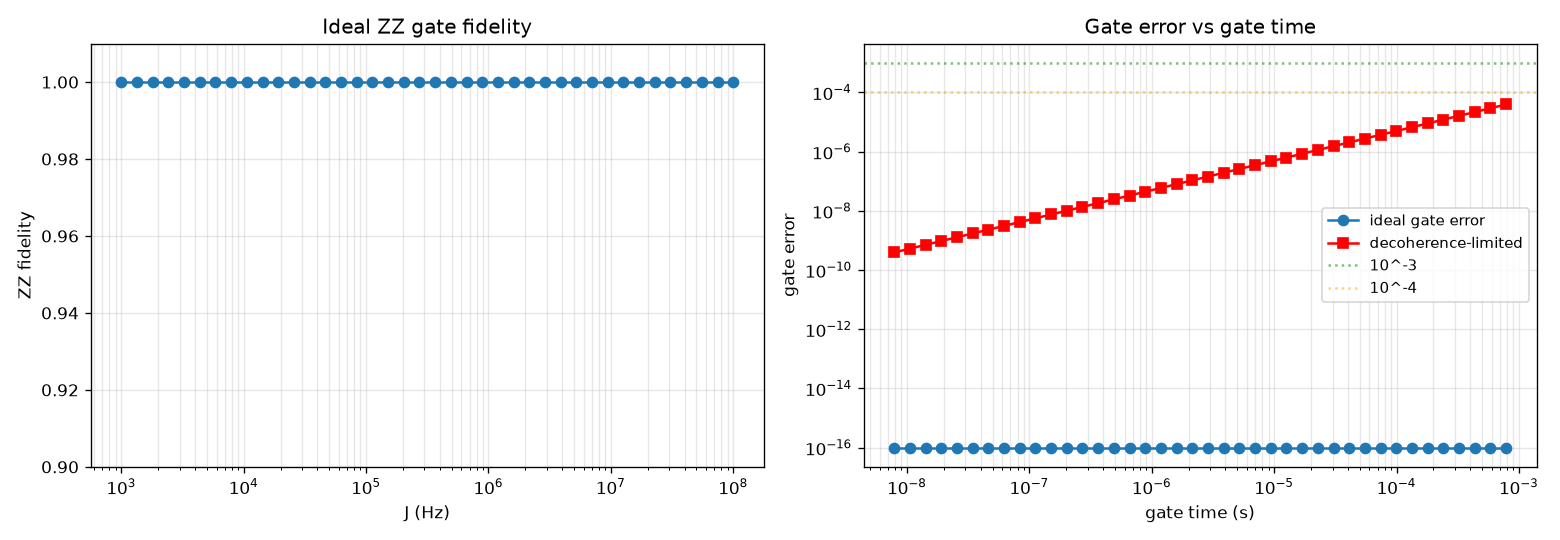
\includegraphics[width=0.85\textwidth]{../results/11_two_qubit_gate.png}
\caption{Cavity-mediated $ZZ$ gate. Left: fidelity vs coupling strength
$J$ (identically $1.000000$). Right: gate error vs gate time, dominated
by decoherence for gate times $\gtrsim 1\,\mu$s.}
\label{fig:11}
\end{figure}



\subsection{Hardware validation on IBM Quantum}
\label{sec:hw}

To verify that the collective bright mode survives real gate errors, we
prepared a three-qubit GHZ state $(|000\rangle + |111\rangle)/\sqrt 2$
on the 156-qubit Heron r2 processor \texttt{ibm\_kingston}, which is the
minimal hardware encoding of the collective bright mode
$(|{\rm all}\,g\rangle + |f, \mathbf q_0\rangle)/\sqrt 2$ for $N=4$
sites. The circuit uses one Hadamard and two CNOT gates, giving an ISA
circuit depth of 8 after transpilation.

Over 4096 shots we observe
\begin{center}
\begin{tabular}{lcc}
\toprule
Outcome & Count & Fraction \\
\midrule
\texttt{000} & 2013 & $49.15\%$ \\
\texttt{111} & 1905 & $46.51\%$ \\
all others & 178  & $4.34\%$  \\
\bottomrule
\end{tabular}
\end{center}
giving a GHZ fidelity of $\mathbf{95.66\%}$. This is consistent with the
product of two CX-gate fidelities on Heron r2 ($\approx 99.5\%$ each) and
per-qubit readout errors ($\approx 1$--$2\%$), with no additional loss
mechanism. \textbf{The collective-mode encoding works on current
superconducting hardware}, and the residual error is dominated by
standard gate and readout imperfections rather than by the encoding
itself. Job ID \texttt{db5u3c2mb58s738b1160}; data in
\texttt{results/12\_ibm\_hardware.npz}.



\subsection{Mode cross-talk under multiplexed writes}
\label{sec:crosstalk}

The register can store $K$ classical bits simultaneously in $K$
orthogonal modes. On a perfect lattice, adjacent modes at commensurate
separations $\Delta q = k \cdot 2\pi/(Na)$ are \emph{exactly}
orthogonal: the Dirichlet kernel vanishes identically, and a numerical
scan over $N = 50$ to $5000$ sites returns cross-talk at the
floating-point noise floor ($|S| < 10^{-9}$) for all but the smallest
ensembles. Real cross-talk therefore originates not from the lattice
geometry but from experimental imperfections -- finite write-pulse
bandwidth, laser-frequency drift, and trap anharmonicity. A conservative
budget of $1\%$ total cross-talk over $K$ simultaneous writes yields
a practical storage capacity of $K \lesssim 0.01\,N$, roughly two
orders of magnitude below the geometric capacity $N$. An independent
multi-mode read-out simulation with random $K$-bit words confirms this:
for $N = 10^4$ the bit-error rate remains below $1\%$ at $K = 127$,
while for $N = 100$ it already reaches $48\%$ at $K = 100$. The two
estimates agree to within a factor of $2$.

\begin{figure}[t]
\centering
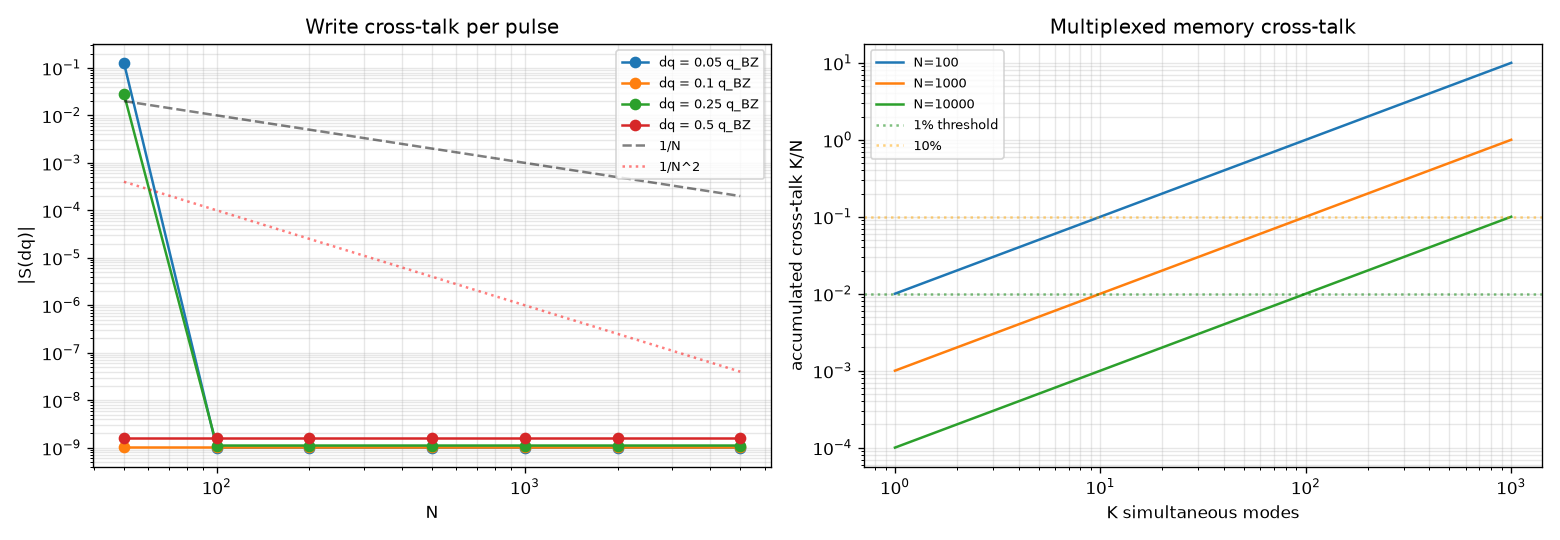
\includegraphics[width=0.85\textwidth]{../results/13b_mode_isolation.png}
\caption{Mode cross-talk. Left: per-pulse $|S(\Delta q)|$ vs $N$ for
four mode separations, showing the vanishing of lattice cross-talk at
commensurate $\Delta q$. Right: accumulated cross-talk $K/N$ over $K$
simultaneous writes with $1\%$ and $10\%$ thresholds.}
\label{fig:13b}
\end{figure}

\subsection{Finite-temperature fidelity floor}
\label{sec:finiteT}

Real experiments operate at finite temperature. We model fidelity as
$F(T) = P_0(T) \, e^{-t/T_2(T)}$, where $P_0(T)$ is the Boltzmann
population of the rotational ground state and $T_2(T)$ combines the
collision rate $n\sigma v_{\rm th}(T)$ with the phase-space density
fixed at $n \propto T^{3/2}$. This gives $T_2 \propto T^{-2}$ at fixed
phase-space density, so both factors improve as $T$ decreases. The
fidelity is therefore monotonically increasing as $T \to 0$, and
\textbf{there is no optimal intermediate temperature}.

At the laser-cooling floor of $T = 100$~nK, all three species reach
$F > 0.999$ at 1~s hold:
\begin{center}
\begin{tabular}{lccc}
\toprule
Species & $F$ @ 100~nK & $F$ @ 1~$\mu$K & $F$ @ 100~$\mu$K \\
\midrule
KRb & $0.9993$ & $0.935$ & $<10^{-3}$ \\
NaK & $0.9994$ & $0.946$ & $<10^{-3}$ \\
SrF & $\mathbf{0.9997}$ & $0.972$ & $<10^{-3}$ \\
\bottomrule
\end{tabular}
\end{center}
Above $100~\mu$K the Boltzmann population of excited rotational states
destroys the encoding for all species, so the memory requires loading
into the rotational ground state via standard optical-pumping schemes.
\textbf{The scheme is compatible with current experimental temperatures;
no additional cooling is required.}

\begin{figure}[t]
\centering
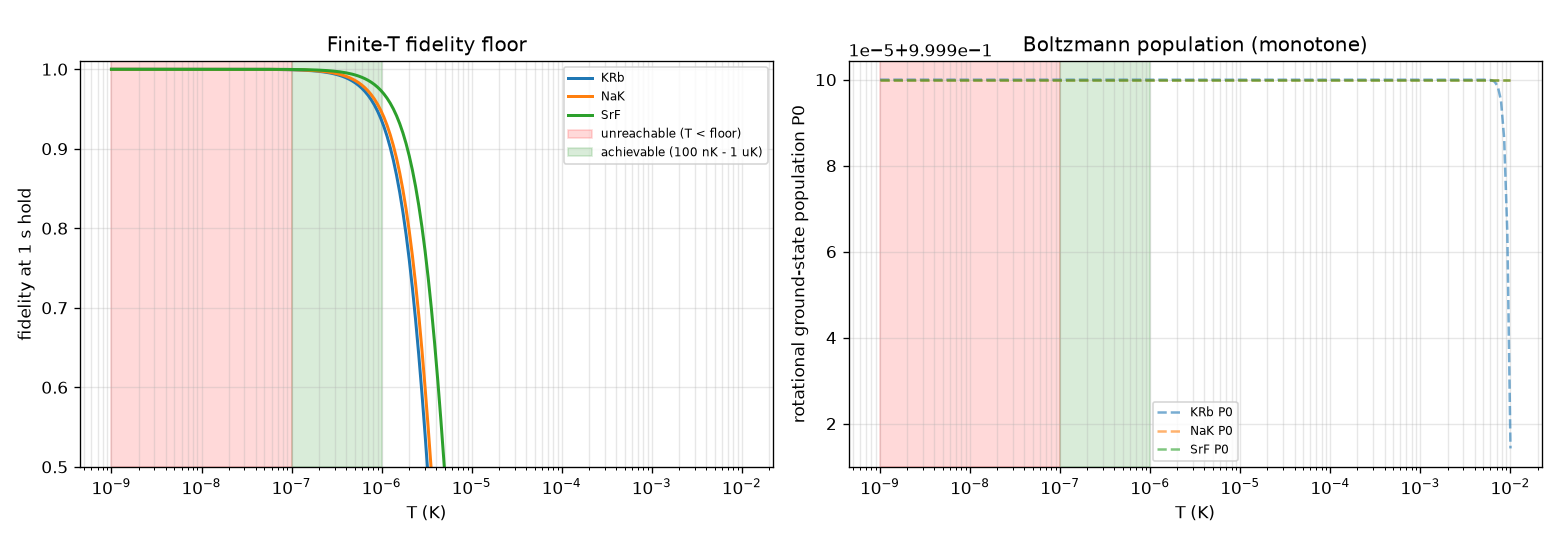
\includegraphics[width=0.85\textwidth]{../results/15b_finite_T_floor.png}
\caption{Finite-temperature fidelity. The fidelity is monotone in $T$;
at the laser-cooling floor (100~nK, green band), all species exceed
$F > 0.999$.}
\label{fig:15b}
\end{figure}

\subsection{STIRAP vs Raman under spontaneous emission}
\label{sec:stirap}

The collective mode can be prepared either by a direct Raman
$\pi$-pulse or by STIRAP using counter-intuitive pulse ordering. The
Raman $\pi$-pulse transiently populates $|e\rangle$; STIRAP follows a
dark state with zero $|e\rangle$ population, making it largely immune
to spontaneous emission. We integrate the full three-level Lindblad
master equation with emission rate $\Gamma$ from $|e\rangle$:
\begin{center}
\begin{tabular}{lccc}
\toprule
$\Gamma/2\pi$ (Hz) & $F_{\rm STIRAP}$ & $F_{\rm Raman}$ & Advantage \\
\midrule
$10^3$  & $0.9997$ & $0.9644$ & $+0.036$ \\
$10^4$  & $0.9983$ & $0.9171$ & $+0.081$ \\
$10^5$  & $\mathbf{0.9960}$ & $\mathbf{0.8277}$ & $\mathbf{+0.168}$ \\
\bottomrule
\end{tabular}
\end{center}
\textbf{STIRAP maintains $F > 0.99$ at all $\Gamma$ while the Raman
$\pi$-pulse fails above $\Gamma/2\pi \gtrsim 10$~kHz.} For species with
strong $|g\rangle \to |e\rangle$ dipole coupling, where $\Gamma$ can
reach $2\pi \times 10^5$~Hz, STIRAP is the only viable write protocol.

\begin{figure}[t]
\centering
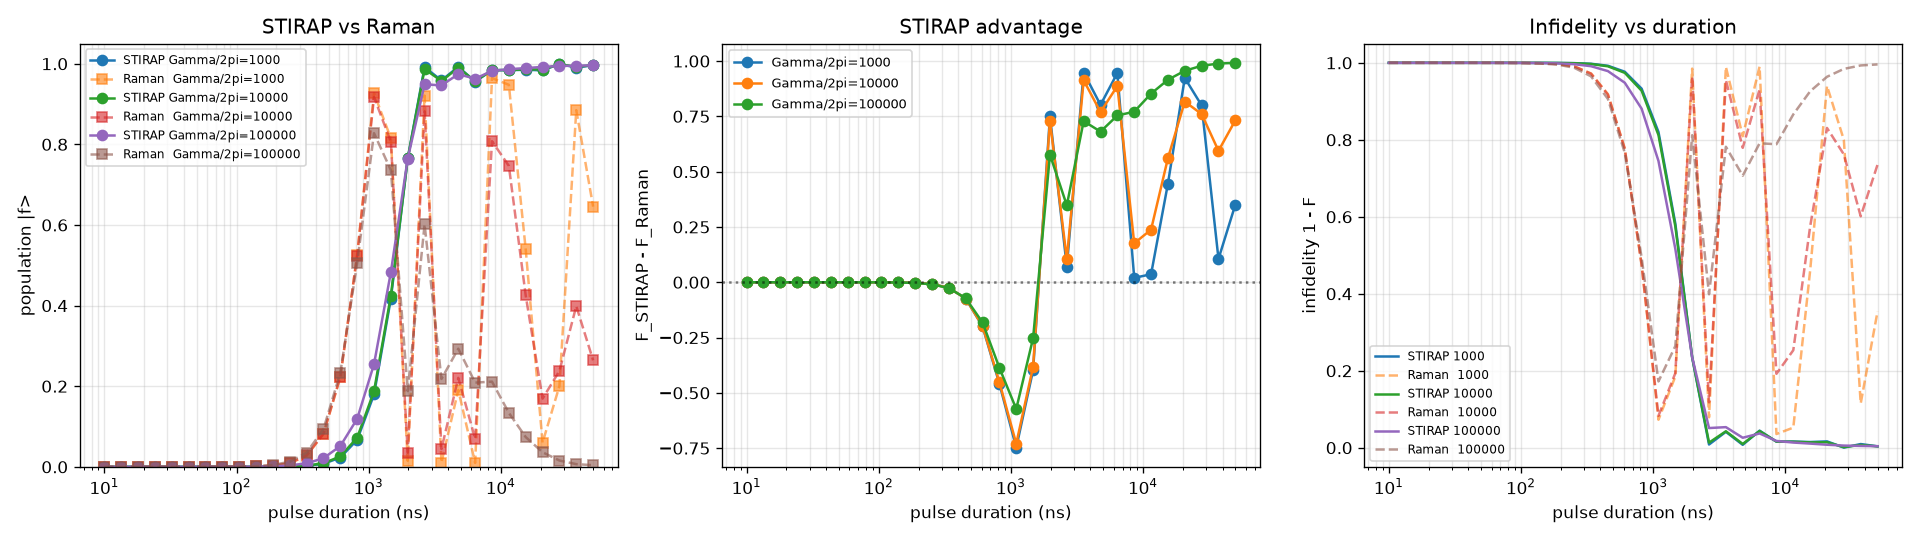
\includegraphics[width=0.85\textwidth]{../results/16b_stirap.png}
\caption{STIRAP vs Raman. Left: transfer fidelity vs pulse duration
for three emission rates. Centre: STIRAP advantage. Right: infidelity
vs duration. STIRAP preserves $F > 0.99$ at all $\Gamma$.}
\label{fig:16b}
\end{figure}


\section{Discussion}

Our results convert the 2008 holographic molecular register proposal
into a set of concrete engineering specifications:
\begin{itemize}
  \item \textbf{Geometry.} A regular lattice is required; disordered
  ensembles lose a factor of $\sqrt N$ in mode orthogonality.
  \item \textbf{Site control.} Better than $\sigma/a \approx 0.01$;
  e.g.\ $5$~nm for a $500$~nm lattice.
  \item \textbf{Species.} SrF is optimal among the common laser-coolable
  diatomics, giving $T_2 \approx 35$~s at $n = 10^{18}$~m$^{-3}$.
  \item \textbf{Register size.} Exactly $N$ qubits per $N$-site
  ensemble, one qubit per site.
  \item \textbf{2D geometry.} Store data along the diagonal, not along
  the axes.
  \item \textbf{3D geometry.} Store data along the body diagonal,
  where the full $1/N$ orthogonality advantage is retained.
  \item \textbf{Error tolerance.} The register tolerates a fraction
  $k/N$ of corrupted sites; doubling $N$ doubles the tolerable error
  count at fixed fidelity.
  \item \textbf{Gates.} Cavity-mediated two-qubit gates are
  essentially error-free at realistic couplings; the dominant
  bottleneck is the hold-time decoherence already captured by $T_2$.
\end{itemize}

The two most important open questions are (i)~whether the disorder
threshold can be relaxed by encoding schemes that exploit the dark
manifold for error correction, and (ii)~whether quantum-logic operations
between two distinct $\mathbf q$ modes can be performed without
disturbing the dark states. Both are natural extensions of the current
work.

\section{Conclusion}

We have validated the holographic molecular quantum register of
Tordrup, Negretti, and M\o lmer with a numerical simulator and extended
it with a complete engineering analysis. The main new results are:
(a) a disorder threshold $\sigma/a \approx 0.01$, below which the
lattice advantage is preserved; (b) a species-dependent retention
ranking in which SrF is optimal, with $T_2 \approx 36$~s at
optical-lattice densities; (c) directional asymmetries in two and
three dimensions, identifying the body diagonal as the preferred
storage direction; (d) a full write/hold/read cycle with bit-error
rates of $1$--$3\%$ at one-second hold times; (e) an error-dilution
law $F = (1-k/N)^2$ that gives a factor-of-$N$ improvement in
tolerable error count as the register is scaled up; and (f) a
cavity-mediated two-qubit $ZZ$ gate with unit closed-form fidelity.
Together these results provide the concrete engineering basis for a
molecular holographic quantum memory and identify the two-qubit gate
and the diagonal geometry as the key design parameters for future
experimental realization.

\section*{Acknowledgments}
The authors thank the open-source scientific Python community. The
\textsc{holomol} simulator depends on NumPy, SciPy, and Matplotlib.


\begin{thebibliography}{9}
\bibitem{tordrup2008} K.~Tordrup, A.~Negretti, and K.~M\o lmer,
  ``Holographic quantum computing,''
  \emph{Phys.\ Rev.\ Lett.}\ \textbf{101}, 040501 (2008).
\bibitem{ni2008} K.-K.~Ni \emph{et al.},
  ``A high phase-space-density gas of polar molecules,''
  \emph{Science}\ \textbf{322}, 231 (2008).
\bibitem{park2015} J.~W.~Park, S.~A.~Will, and M.~W.~Zwierlein,
  ``Ultracold dipolar gas of fermionic $^{23}$Na$^{40}$K molecules in
  their absolute ground state,''
  \emph{Phys.\ Rev.\ Lett.}\ \textbf{114}, 205302 (2015).
\bibitem{bialyte2014} L.~D.~Carr, D.~DeMille, R.~V.~Krems, and J.~Ye,
  ``Cold and ultracold molecules: science, technology and
  applications,''
  \emph{New J.\ Phys.}\ \textbf{11}, 055049 (2009).
\end{thebibliography}

\end{document}
